%%%%%%%%%%%%%%%%%%%%%%%%%%%%%%%%%%%%%%%%%%%%%%%
%%% Template for lab reports used at STIMA
%%%%%%%%%%%%%%%%%%%%%%%%%%%%%%%%%%%%%%%%%%%%%%%

%%%%%%%%%%%%%%%%%%%%%%%%%%%%%% Sets the document class for the document
% Openany is added to remove the book style of starting every new chapter on an odd page (not needed for reports)
\documentclass[10pt,english, openany]{book}

%%%%%%%%%%%%%%%%%%%%%%%%%%%%%% Loading packages that alter the style
\usepackage{graphicx}
\usepackage{subcaption}
\usepackage[]{color}
\usepackage{alltt}
\usepackage[T1]{fontenc}
\usepackage[utf8]{inputenc}
\usepackage{amsfonts}
\usepackage{amsmath}
\usepackage{mathtools}
\setcounter{secnumdepth}{3}
\setcounter{tocdepth}{3}
\setlength{\parskip}{\smallskipamount}
\setlength{\parindent}{0pt}

% Set page margins
\usepackage[top=100pt,bottom=100pt,left=68pt,right=66pt]{geometry}

% Prevents LaTeX from filling out a page to the bottom
\raggedbottom

% Adding both languages
\usepackage[english, italian]{babel}

% All page numbers positioned at the bottom of the page
\usepackage{fancyhdr}
\fancyhf{} % clear all header and footers
\fancyfoot[C]{\thepage}
\renewcommand{\headrulewidth}{0pt} % remove the header rule
\pagestyle{fancy}

% Changes the style of chapter headings
%\usepackage{titlesec}
% \usepackage[Glenn]{fncychap}
% Adds table captions above the table per default
\usepackage{float}
\floatstyle{plaintop}
\restylefloat{table}

% Adds space between caption and table
\usepackage[tableposition=top]{caption}

% Adds hyperlinks to references and ToC
\usepackage{cite}
\usepackage{hyperref}
\hypersetup{hidelinks,linkcolor = black} % Changes the link color to black and hides the hideous red border that usually is created

% If multiple images are to be added, a folder (path) with all the images can be added here 
\graphicspath{ {Figures/} }

% Algorithms
\usepackage[ruled,vlined]{algorithm2e}

\newtheorem{definition}{Definition}
\DeclarePairedDelimiter\abs{\lvert}{\rvert}



% Separates the first part of the report/thesis in Roman numerals
\frontmatter
%%%%%%%%%%%%%%%%%%%%%%%%%%%%%% Starts the document
\begin{document}

%%% Selects the language to be used for the first couple of pages
\selectlanguage{english}

\author{Julian Eßer}
\title{Personal Lecture Notes \\
MITx6.832x: Underactuated Robotics \\
(Spring 2019) \\
{\Large Algorithms for Walking, Running, Swimming, Flying, and Manipulation}}

%%%%% Adds the title page
\begin{titlepage}
\maketitle
\end{titlepage}

% Adds a table of contents
\tableofcontents{}

%%%%%%%%%%%%%%%%%%%%%%%%%%%%%%%%%%%%%%%%%%%%%%%%%%%%%%%%%%%%%%%%%%%%%%%%%%%%%%%%%%%%%%%%%%%%
%%%%%%%%%%%%%%%%%%%%%%%%%%%%%%%%%%%%%%%%%%%%%%%%%%%%%%%%%%%%%%%%%%%%%%%%%%%%%%%%%%%%%%%%%%%%
%%%%% Text body starts here!
\mainmatter

\chapter{Introduction}\label{chapt:intro}
The purpose of this document is to provide a brief overview of the essential knowledge of the underactuated robotics class \cite{mitx6.832web} from MIT taught in Spring 2019. Special emphasis is on the following topics:\\
\begin{itemize}
\item Understanding Control as Optimization
\item Dynamics of Biped Locomotion
\item Optimization of Biped Locomotion
\end{itemize}

\chapter{Lecture 1: Why Study Robot Dynamics?}\label{lecture1}
\section{Background / Motivation}
The \textbf{motivation} for this course is to
\begin{itemize}
\item Build great robots that can do amazing things
\item Exploit natural dynamics of robots, not just doing dump control
\item Achieve extraordinary performance in terms of speed, efficiency, or robustness (Honda's ASIMO vs. passive dynamic walkers)
\item Controlling nonlinear systems without complete control authority
\item View computation of challenging tasks in robotics (manipulation, autonomous driving) through the lense of dynamics.
\end{itemize}
This course is all about nonlinear dynamics and control of underactuated mechanical systems, with an emphasis on computational methods. Especially it covers the \textbf{topics}
\begin{itemize}
\item Nonlinear dynamics
\item Applied optimal and robust control
\item Motion planning
\item Examples from biology and applications to legged locomotion, compliant manipulation, underwater robots, and flying machines
\end{itemize}

\section{Definitions}
Nonlinear differential equations typically take the form
$$ \dot{x} = f(x,u) $$
where $f$ is a vector valued function, $x$ is the state vector and $u$ is the vector of control input and $\dot{x}=\frac{dx}{dt}$ is the time derivative.
Mechanical Systems are described by second order differential equations. When the state vector is defined as 
$$x=\begin{bmatrix}q \\ \dot{q}\end{bmatrix},$$ 
where the system dynamics can be described as
$$\ddot{q}=f(q,\dot{q}, u).$$
Since mechanical systems are \textit{control affine}, this specializes to
$$ \ddot{q}=f_{1}(q,\dot{q})+f_{2}(q,\dot{q})u.$$
A system of this form is called \textit{underactuated} if $rank[f_{2}]<=n$. 
Other causes of underactuated include
\begin{itemize}
\item Input saturation (e.g. torque limits)
\item State constraints (e.g. joint limits)
\item Model uncertainty / state estimation
\end{itemize}
 
\section{Manipulator Equations}
The equations of motion for simple systems, e.g. a double pendulum, are quite simple to derive. Results, e.g. obtained from an Lagrangian calculation approach, can be expressed in the form of the standard "manipulator equations":
$$M(q)\ddot{q}+C(q,\dot{q})\ddot{q}=\tau_{g}(q)+Bu$$ 
where $M$ is the Inertia matrix, $C$ is the matrix of Coriolis terms $\tau_{g}$ covers gravitational torques, $B$ maps inputs to generalized force and u is the control input (either force or torque).

The acceleration then is expressed as
\begin{equation}\label{eq:eom_dbl_pendl}
\ddot{q}=M^{-1}(q)[\tau_{g}(q)+Bu-C(q,\dot{q})\dot{q}].
\end{equation}
With equation \ref{eq:eom_dbl_pendl}, the dynamics of the systems and accordingly the functions $f_{1}$ and $f_{2}$ are fully defined.

For simulating the dynamics of a robot, it is sufficient to provide the  kinematics in form of a \textit{URDF file}, pass it to an forward Dynamics solver and you get the resulting acceleration and its integrations.

\section{Plan for the Course}

\begin{figure}[h!]
\begin{center}
  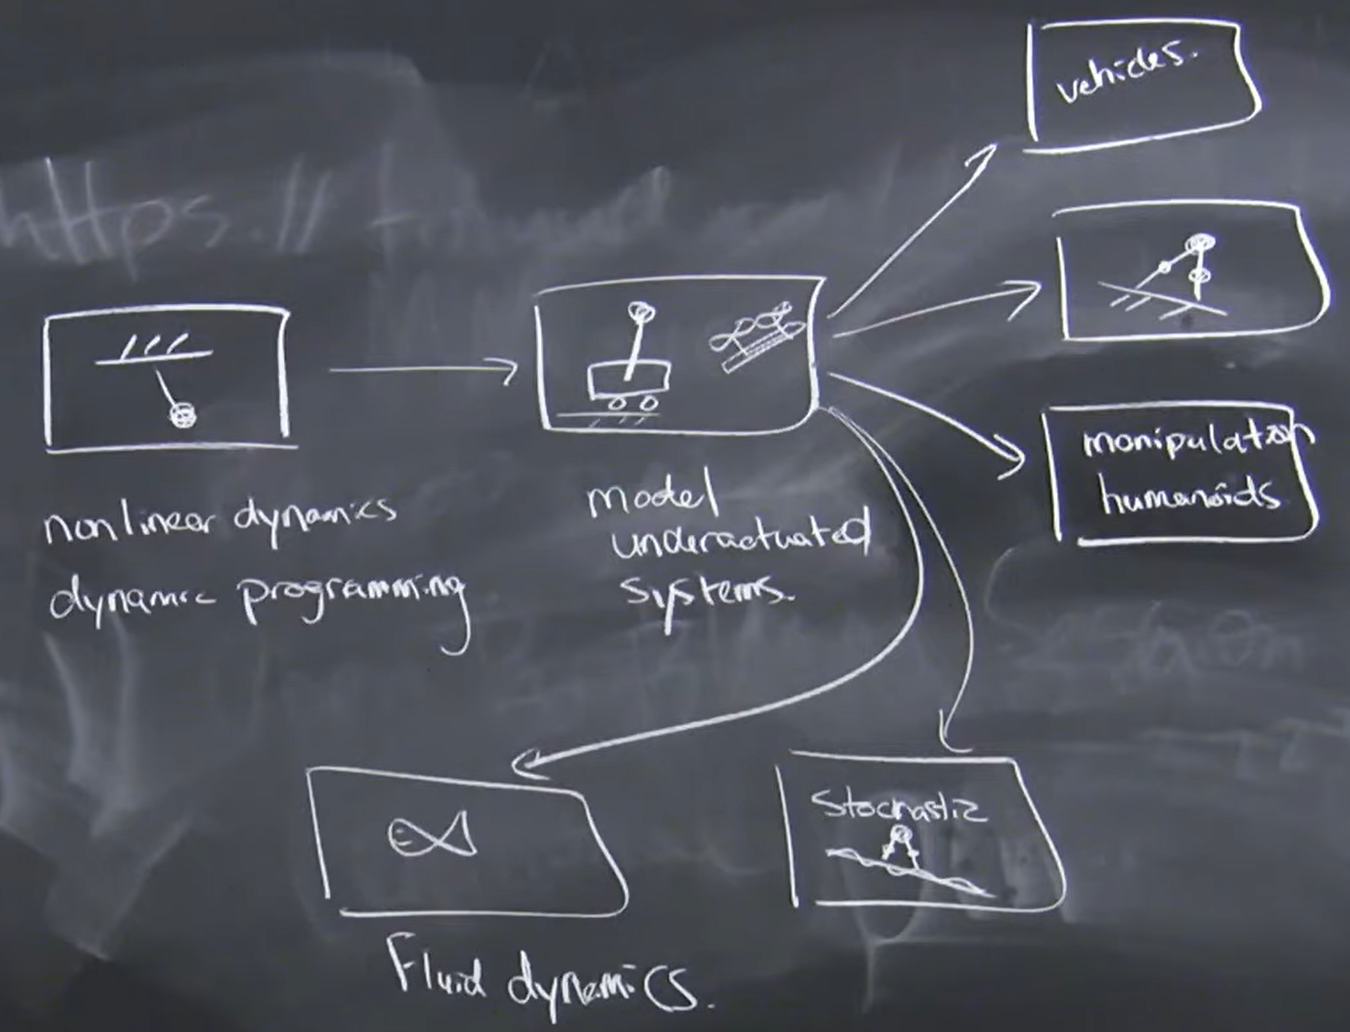
\includegraphics[width=1\textwidth]{Figures/courseOverview.png}
  \caption{Course overview: Basics first, then simple systems and then various advanced systems.}
  \label{fig:overview}
\end{center}
\end{figure}
\chapter{Lecture 2: Nonlinear Dynamics}\label{lecture2}
\section{The Simple Pendulum}
Even the most simple dynamical systems, e.g. the simple pendulum, can not be solved in a closed form. This is due to the nonlinear characteristics of the underlaying differential equations. But actually you don't have to in order to describe and analyse fundamental dynamical characteristics. 

But what we really care about is the long-term behaviour of the sytem. For low dimensional systems, two central tools are available in order to analyse the systems behaviour: 
\begin{itemize}
\item Linearization
\item Graphical Analysis
\end{itemize}
 
The equations of motion of the simple pendulum can be derived with the Langrangian as:
$$ ml^2 \ddot\theta(t) + mgl\sin{\theta(t)} = Q $$ 
Considering the generalized force $Q$ as combination of damping and a control torque input
$$ Q = -b\dot\theta(t) +u(t).$$
For the case of a constant torque this yields
$$ ml^2 \ddot\theta + b\dot\theta + mgl \sin\theta = u_0.$$

\section{Graphical Analysis}
\subsection{Fixed Points}
The central goal of control is to meaninfully shift the vector field via sophisticated control input of a system in order to change its dynamics.  
So called \textit{phase plots} are useful for visualizing this vector field of two-dimensional systems.  In case of the state vector $x= \begin{bmatrix} \theta \\ \dot{\theta} \end{bmatrix}$ this means $\dot{\theta}$ over $\theta$.

\begin{definition}
A point the system will remain forever without applying external forces is called a fixed point or a steady state respectively.
\end{definition}
The position of fixed points, e.g. stable positions of the pendulum, strongly depend on the parameter of the system (damping, input torque etc.). 

\subsection{Definitions of Stability}
There are existing different types of stability in order to describe the behaviour next a fixed point $x^{\star}$. The fixed point can be 
\begin{itemize}
\item \textit{Stable} in the sense of Lyapunov (i.e. will remain within certain radius)
\item \textit{Asymptotically stable} (i.e. for $t->\infty$ reaches certain point)
\item \textit{Exponentially stable} (reaches certain point at defined rate).
\end{itemize}

\chapter{Lecture 3: Dynamic Programming I}\label{lecture3}
\section{Control as Optimization}
\begin{itemize}
\item The big idea is to formulate control design as an optimization problem.
\item Given a trajectory $x(.),u(.)$ we want to assign a score (scalar) to decribe the performance.
\item Additionally we can set constraints in order to exclude trajectories that exceed certain limits (e.g. control limit $\abs{u(t)}<=1$).
\item The goal is to find a control policy $u=\Pi(t,x)$ that optimizes that score!
\item When solving optimal control problems, one most often needs numerical approximation.
\end{itemize}
The strengths of Optimal Control are that it
\begin{itemize}
\item is a very general approach; it can be applied to fully/underactuated, linear/nonlinear systems,
\item contains an very intuitive approach by describing just the goal and some constraints 
\item works very well with numerical approximation.

\end{itemize}
 
 
\section{Example: Double Integrator}\begin{itemize}
\item Very simple example that can be solved without numerical approximation.
\item Consists of "brick of ice" on a flat floor
\item Goal: Go to origin as fast as possible
\end{itemize}
Easiest case: Formulate optimal control as "Bang-Bang". Accelerate (full throttle) then slam on the brakes.


\section{Dynamic Programming Algorithm}
\subsection{Discrete Time Space: Optimal Control as Graph Search}
For systems with a finite, discrete set of states and a finite, discrete set of actions, dynamic programming also represents a set of very efficient numerical algorithms which can compute optimal feedback controllers.

Cost function
$$one-step cost: g(s,a)$$
$$total cost: \sum_{n=0}^{\infty} $$
Key idea: Additive cost 
$$\int_0^T g(x(t),u(t)) dt,$$
There are existing numerous possibilities on how to design the cost function:
\begin{itemize}
\item Min-time: $g(s,a) = 1 "if" s~=s_{goal}; 0 if otherwise$
\item Quadratic cost: $g(x,u)=x^{T}x+u^{T}u$
\end{itemize}
There are many algorithms for finding (or approximating) the optimal path from a start to a goal on directed graphs. In dynamic programming, the key insight is that we can find the shortest path from every node by solving recursively for the optimal cost-to-go (the cost that will be accumulated when running the optimal controller) from every node to the goal.
Recursive form of the optimal control problem:
\begin{equation} \hat{J}^*(s_i) \Leftarrow \min_{a \in A} \left[ \ell(s_i,a) +
    \hat{J}^*\left({f(s_i,a)}\right) \right]
    \end{equation}
If we know the optimal cost-to-go, then it's easy to extract the optimal policy:
\begin{equation} \pi^{*}(s_i) = argmin_a
    \left[ \ell(s_i,a) + J^*\left( f(s_i,a) \right) \right].
\end{equation}

Limitations:
\begin{itemize}
\item Accuracy for continuous systems (discretisation error)
\item Scaling (curse of dimensionality)
\item Assumes full state information: Absolutely not necessary to know everything
\end{itemize}

\subsection{Continous Dynamic Programming}






\section{Numerical Optimal Control of the pendulum}

\include{lecture4}
\include{lecture5}
\include{lecture6}
\include{lecture7}
\include{lecture8}
\include{lecture9}
\include{lecture10}












































\pagebreak
% Adding a bibliography if citations are used in the report
\bibliographystyle{plain}
\bibliography{../commonBibFile.bib}
% Adds reference to the Bibliography in the ToC
\addcontentsline{toc}{chapter}{\bibname}

\pagebreak



\end{document}
